%% LyX 2.0.7 created this file.  For more info, see http://www.lyx.org/.
%% Do not edit unless you really know what you are doing.
\documentclass[11pt,twocolumn]{article}
\usepackage[utf8]{inputenc}
\usepackage{graphicx}

\makeatletter
%%%%%%%%%%%%%%%%%%%%%%%%%%%%%% User specified LaTeX commands.




\title{Smarter Merge Tool for Structured Java Code }
\author{Kartik Andalam, Raoul D'Cunha, Shreya Shah }
\date{March 2014}

\makeatother

\begin{document}
\maketitle

%\twocolumn



\section{Abstract}

Software merging is a necessity for large-scale software development
and while there are many code version systems to help with this, many
of them don't take the structure of the code into account. Understanding
the semantic and the syntactic structure of the code helps automate
merging further, which in turn requires less effort from the developer
at commit.

We propose a tool that would attempt to automate merging and also
assist the user in identifying the changes by analysing the semantics
of the code. We intend to use PDStore%
\footnote{PDStore is a Triplestore database developed at the University of Auckland%
} to store the code in a structured manner that can be used in a versioning
system. The proposal also highlights the requirements, milestones
and possible evaluation methods for the research project.


\section{Motivation}

Today's code version systems are based on textual comparisons. Being
textual based means that they do not understand the structure of the
code, and as a result the tools are unable to assist the developer
with code merging. This gave motivation to utilise the extra information
that can aid in the merging.

We aim to develop a language-aware code versioning system based on
PDStore. In particular, we will utilize structured data to visualize
changes to the structure of a source code file to assist with merging.


\section{Related Work}

\cite{CodeClones} proposes a novel method for merging code clones
and presents a successful case study conducted by using the Aries
tool which uses to identify code clones and merge them. The method
described in \cite{CodeClones} consists of a two phase process, where
code clones that can be refactored are quickly detected, and the metrics
are measured which indicate how the detected code clones should be
merged.

\cite{SemanticDiff} describes a tool called “Semantic diff” and techniques
used in that tool to show the effect of modifications. The tool aims
at providing the user with a summarised report of semantic changes
between two versions of a procedure, and focuses on minimising any
spurious differences such as, renaming local variables. While the
tool provides knowledge of variable dependences within a procedure,
it is not very helpful when considering an entire program because
the tool does not maintain any relationship between method invocation
and method definition.

In \cite{XMLMerge} a technique for performing a 3 way structured
XML merge is described. The technique involves defining merge rules
derived from common use cases of XML editing. While there are similar
problems, a few differences exist. By the nature of XML, the local
structure is important. However with Java code the structure can vary
and still present the same semantic definition. Thus some of the rules
made in \cite{XMLMerge} become invalid for flexible structured data
such as code.

\cite{mergegraph} describes the problems associated with common textual
based merging. It proposes a solution that can be applied to software
artefacts of different types. The solution involves representing information
with extra information such as namespaces appended with UIDs. Once
the data is represented in this special structure, the job of analysing
two structures should be made easier.


\section{Requirements}

A successful execution of the research endeavour should meet the following
requirements: 
\begin{enumerate}
\item To be able to successfully identify simple changes in method body
but not necessarily code structure 
\item To be able to successfully identify and common sections of code in
two structures with slight variations 
\item Identify changes in structure, such as method location being shifted 
\item Successfully merge two differing versions of code following from the
examples in 1 and 2 
\end{enumerate}
The following optional requirements would also be attempted to met
during the execution of this research endeavour 
\begin{enumerate}
\item To integrate this additional functionality into the existing PDStore
versioning application. 
\end{enumerate}

\section{Design and Implementation}

The underlying technology used in the proposed method involves using
PDStore to be able to form a structured view of the code. The logic
for doing the detection and merging will be written in Scala. After
defining a method to define “sameness” of a section of the code, we
will be using a similar approach to \cite{XMLMerge} to generate rules
that help define merging.

The following describes an example of where our tool successfully
merges two documents, identifying the changes with respect to semantic
meaning and structure.

Figure 1 shows one possible scenario we intend to solve with our tool.
We aim to recognise if a method is carrying out the same procedure
as an existing method, at commit. As you can see in the above figure,
the tool merges the two methods into one, by keeping the recent name
of the method and same code within the method.

\begin{figure}
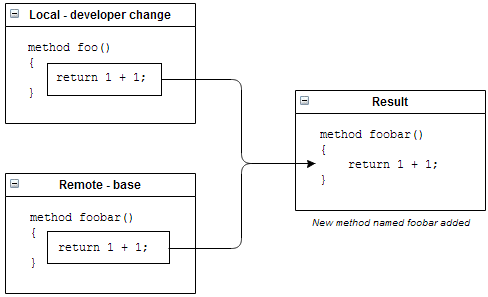
\includegraphics[scale=0.44]{IdentificationOfChanges}\caption{Identification of changes and merged result}
\end{figure}



\section{Evaluation}

Paper prototypes will be used to evaluate the feasibility of the User
Interface design of our tool. This study will reveal both fundamental
and minor flaws in the UI that would need to be fixed before the final
milestone. Specific scenarios will be constructed outlining various
use cases that will then be run through by the participants on multiple
different UI designs. The participants will be asked to think out
loud, so that their thought process can be observed and evaluated.
Feedback will then be collected from the participants at the end through
the use of a questionnaire which will then be used to measure the
usefulness of each design.

Any flaws which are identified will then be corrected and the test
will then be undertaken again so as to verify that the flaws are indeed
fixed.


\section{Project Plan}

Listed below are the three milestones for this project %\newline adding a new line puts too much space over here

\begin{description}
\item [{Milestone One:}] Successfully identify the type of simple structural
changes


This involves defining rules and defining a notion of “sameness” for
two code artefacts. The PDStore database will be used to compare the
two different versions of the code. Completion criteria involves being
able to generate output that clearly identify the changes. \\
 \textbf{Due Date:} 15th April 2014

\item [{Milestone Two:}] Perform merging of simple structural changes


After being able to identify the changes, we need to define appropriate
rules for merging. To complete the milestone, the merger will be required
to successfully merge files for a few defined scenarios. \\
 \textbf{Due Date:} 30th April 2014

\item [{Milestone Three:}] Integrate the added functionality to existing
PDStore based versioning tool~


Integrating the added functionality will allow us to conduct our evaluation
on users. This will be key in determining the usefulness and effectiveness
of the changes.\\
 \textbf{Due Date:} 12th May 2014

\end{description}
 \bibliographystyle{plain}
\bibliography{myBib}

\end{document}
